\documentclass{article}

\usepackage{hyperref}
\usepackage{graphicx}
\usepackage{rotating}
\usepackage{pdfpages}


\title{Distributed Artificial Intelligence \\ \large{Report Assignment 5/Lab 8}}
\author{Ewout Pockelé \\ \href{mailto:ewout.pockele@student.uantwerpen.be}{ewout.pockele@student.uantwerpen.be}}


%%%%%%%%%%%%%%%%%%%%%%%%%%%%%%%%%%%%%%%%%%%%%%%%%%%%%%%%%%%%%%%%%%%%%%%%%%%%%%%%


\begin{document}

 \maketitle

 \tableofcontents

 \section[Difference between A2C and PPO]{Difference between Advantage Actor 
   Critic and Proximal Policy Optimizatiom}
 %%%%%%%%%%%%%%%%%%%%%%%%%%%%%%%%%%%%%%%%%%%%%%%%%%%%%%%%%%%%%%%%%%%%%%%%%%%%%%%
  In this section we will describe the differences between Advtantage Actor 
  Critic (A2C) and Proximal Policy Optimization (PPO).

  A2C is an implementation of the more general Actor-Critic method, which tries
  to approximate both the optimal policy and the Q-value function.  A2C is an
  extension that provides (synchronous) parallel learning for the Actor-Critic
  method \cite[p.~62]{mets-policy-gradient}.

  PPO is an extension to the gradient policy learning method that will use
  mulitple epochs of the gradient instead of only the current sample
  \cite[p.~64]{mets-policy-gradient}.

  The most important difference between A2C and PPO is that A2C attempts to
  learn both the optimal policy function and the Q-value function, where PPO
  only tries to learn the optimal policy.  This can be an advantage for PPO in
  situations where the Q-value function might be too complex to effectively
  learn, but has as a disadvantage that, in general, training takes a lot
  longer.

  Another important difference is that PPO is a batched algorithm, while A2C is
  not.  This means that PPO will only update its policy after a whole episode,
  and not during the episode like A2C will.

 \section{Solving the \texttt{LunarLander-v2} environment}
 %%%%%%%%%%%%%%%%%%%%%%%%%%%%%%%%%%%%%%%%%%%%%%%%%%%%%%%%%%%%%%%%%%%%%%%%%%%%%%%
  In this section we will try to solve the \texttt{LunarLander-v2} environment
  from the Gym toolkit\cite{gym}.

  The agents required no modifications from the \texttt{CartPole-v1}
  environment to work on this environment.  As instructed, the variable
  \texttt{N\_TRIALS} was set to $1$ and the variable \texttt{REWARD\_THRESHOLD}
  was set to $100$.

  To tune the parameter \texttt{MAX\_EPISODES}, I first ran the notebook
  without modifying the default value of $500$.  This was enough for the A2C
  agent, which reached the defined threshold in 152 episodes.  The PPO agent
  required significantly more time, taking 2715 episodes to reach the threshold.
  Both these results can be found in \autoref{sec:lunar-notebook}.

 \section[Performance comparison of A2C and PPO]{Performance comparison of 
   Advantage Actor Critic and Proximal Policy Optimization}
 %%%%%%%%%%%%%%%%%%%%%%%%%%%%%%%%%%%%%%%%%%%%%%%%%%%%%%%%%%%%%%%%%%%%%%%%%%%%%%%
  In this section we will be comparing the performance of A2C and PPO in 2
  different environments.

  \subsection{Performance comparison in the \texttt{CartPole-v1} environment}
  \label{subsec:performance-cartpole}
  %%%%%%%%%%%%%%%%%%
   In this section we will compare the A2C agent against the PPO agent in the
   \texttt{CartPole-v1} environment from the Gym toolkit \cite{gym}.

   \begin{figure}[htbp]
    \centering
    \makebox[\textwidth][c]{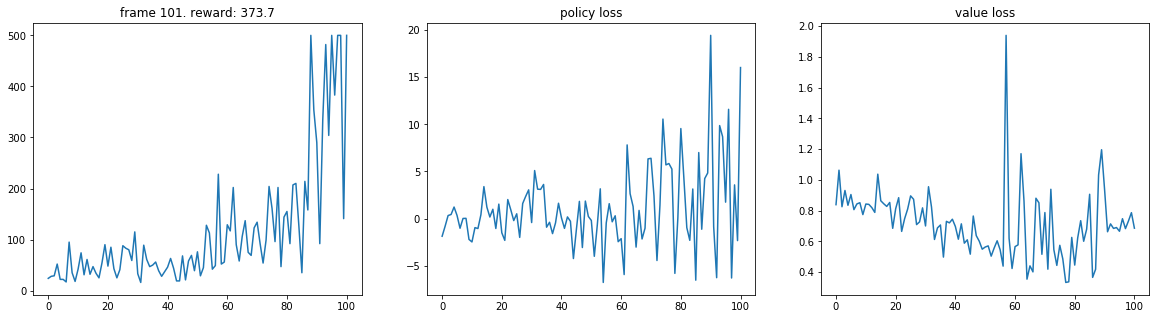
\includegraphics[width=1.5\textwidth]{CartPole-A2C-train}}
    \caption{The reward, policy loss and value loss plots from training the A2C
             agent on the \texttt{CartPole-v1} environment}
    \label{fig:cartpole-a2c-train}
   \end{figure}

   \begin{figure}[htbp]
    \centering
    \makebox[\textwidth][c]{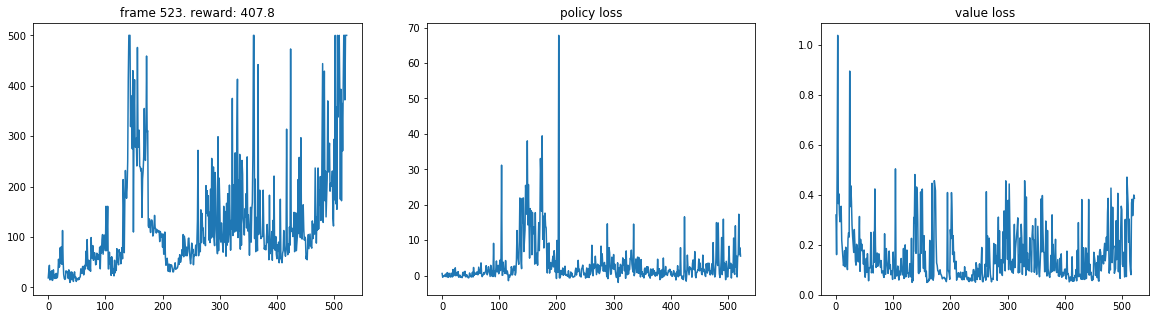
\includegraphics[width=1.5\textwidth]{CartPole-PPO-train}}
    \caption{The reward, policy loss and value loss plots from training the PPO
             agent on the \texttt{CartPole-v1} environment}
    \label{fig:cartpole-ppo-train}
   \end{figure}

   When looking at the A2C agent training statistics in 
   \autoref{fig:cartpole-a2c-train}, and comparing them against the PPO agent
   training statistics in \autoref{fig:cartpole-ppo-train}, we can see that
   training was, apart from the amount of training episodes required, very
   simular.  A notable difference is that the value loss appears to be smaller
   for the PPO agent.  The reward for the PPO agent also seems to have a larger
   variance.

  \subsection{Performance comparison in the \texttt{LunarLander-v2} environment}
  %%%%%%%%%%%%%%%%%%
   In this section I will compare the A2C agent with the PPO agent in the 
   \texttt{LunarLander-v2} environment.
 
   \begin{figure}[htbp]
    \centering
    \makebox[\textwidth][c]{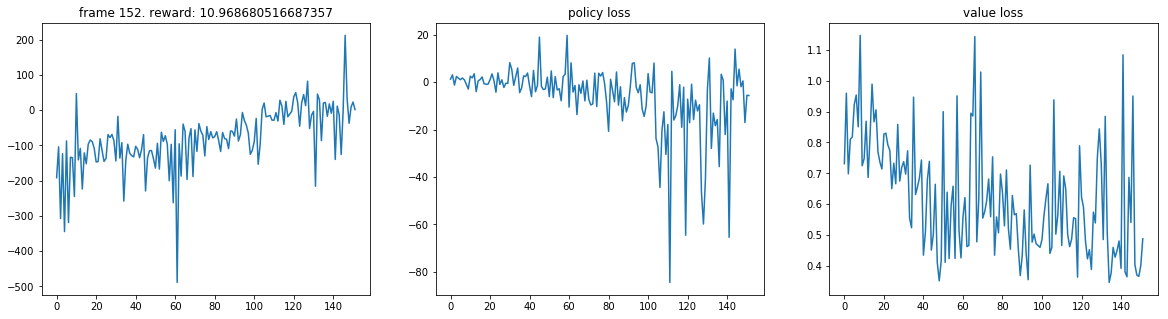
\includegraphics[width=1.5\textwidth]{LunarLander-A2C-train}}
    \caption{The reward, policy loss and value loss plots from training the A2C
             agent on the \texttt{LunarLander-v2} environment.}
    \label{fig:lunar-a2c-train}
   \end{figure}

   \begin{figure}[htbp]
    \centering
    \makebox[\textwidth][c]{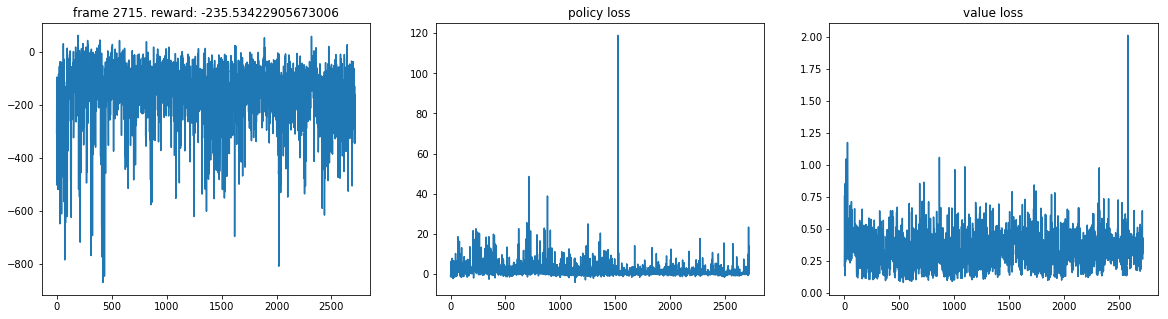
\includegraphics[width=1.5\textwidth]{LunarLander-PPO-train}}
    \caption{The reward, policy loss and value loss plots from training the PPO
             agent on the \texttt{LunarLander-v2} environment.}
    \label{fig:lunar-ppo-train}
   \end{figure}

   When comparing the A2C agent training statistics in 
   \autoref{fig:lunar-a2c-train} with the PPO agent training statistics in 
   \autoref{fig:lunar-ppo-train}, we can see that the PPO agent has much higher 
   peaks for its reward.  When comparing the policy loss graphs, we see 
   someting simular to the \texttt{CartPole-v1} environment, where the policy 
   loss has a simular shape, but it appears to have a bigger variance.  Again 
   like in the \texttt{CartPole-v1} environment, we see that the value loss 
   appears generally lower for PPO then for A2C.

 \section[Analysis of A2C and PPO in different environments]{Analysis of 
   Advantage Actor Critic and Proximal Policy Optimization in different 
   environments}
 %%%%%%%%%%%%%%%%%%%%%%%%%%%%%%%%%%%%%%%%%%%%%%%%%%%%%%%%%%%%%%%%%%%%%%%%%%%%%%%
  In this section I will analyze the performance of A2C and PPO in two
  different environments, the \texttt{CartPole-v1} environment and the
  \texttt{LunarLander-v2} environment.

  \subsection[Analysis of A2C in different environment]{Analysis of Advantage
    Actor Critic in different environments}
  %%%%%%%%%%%%%%%%%%
   In this section I will compare the performance of A2C in 2 different
   environments.

   When comparing the training statistics in \autoref{fig:cartpole-a2c-train}
   and \autoref{fig:lunar-a2c-train}, we can see that the reward in the
   \texttt{LunarLander-v2} environment climbs more gradually, as compared to
   the \texttt{CartPole-v1} environment where after a certain amount of
   training the reward rises rapidly.

   We also see that the policy loss for the \texttt{LunarLander-v2} environment
   is on a bigger scale, even though the (peak) reward is roughly the same
   between them.  In the value loss we see the opposite happening, where the
   value loss in the \texttt{CartPole-v1} environment appears generally higher.

   \begin{figure}[htbp]
    \centering
    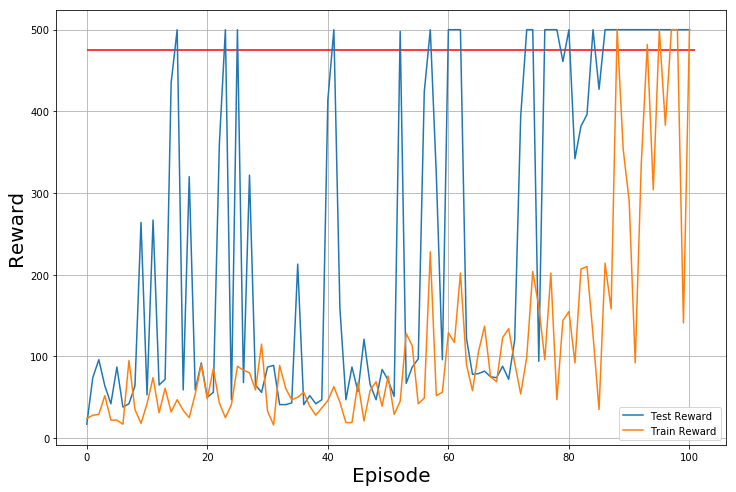
\includegraphics[width=\textwidth]{CartPole-A2C-reward}
    \caption{Rewards of the A2C agent during training in the
             \texttt{CartPole-v1} environment.}
    \label{fig:cartpole-a2c-reward}
   \end{figure}

   \begin{figure}[htbp]
    \centering
    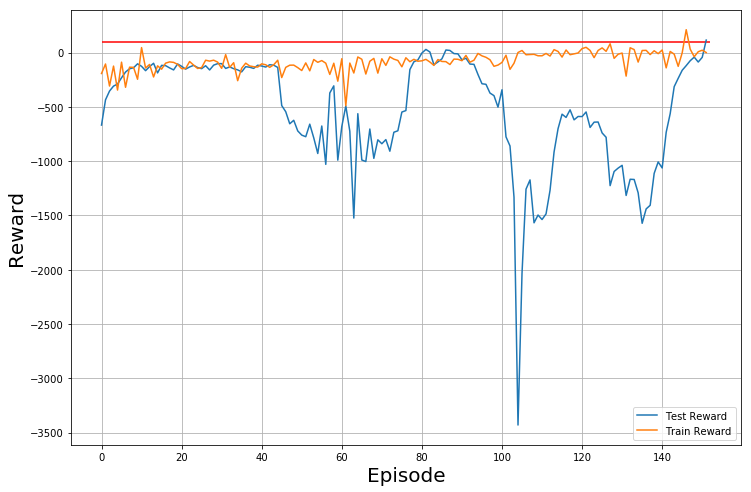
\includegraphics[width=\textwidth]{LunarLander-A2C-reward}
    \caption{Rewards of the A2C agent during training in the
             \texttt{LunarLander-v2} environment.}
    \label{fig:lunar-a2c-reward}
   \end{figure}

   When we go to compare the rewards seen in \autoref{fig:cartpole-a2c-reward}
   and \autoref{fig:lunar-a2c-reward}, we see that the agent for the
   \texttt{CartPole-v1} environment seems to be learning much better, as its
   reward reaches higher rewards more quicker than the training environment.
   In the \texttt{LunarLander-v2} environment we see the opposite happening,
   where the agent scores significantly less in the test environment in some
   episodes.

  \subsection[Analysis of PPO in different environments]{Analysis of Proximal
    Policy Optimization in different environments}
  %%%%%%%%%%%%%%%%%%
   In this section a comparison of the performance of PPO in different
   environments will be made.

   When looking at the statistics in \autoref{fig:cartpole-ppo-train} and
   \autoref{fig:lunar-ppo-train}, we can see that the PPO agent does not seem to
   learn as well on the \texttt{LunarLander-v2} environment as it does on the
   \texttt{CartPole-v1} environment.  This is supported by the fact that
   training took over 5 times as long and both the policy and value losses
   appear significantly higher.  The reward graph also has an interesting shape
   for the \texttt{LunarLander-v2} environment, in that there does not appear to
   be a significant improvement over time.  My guess is that due to the fact 
   that \texttt{N\_TRAILS} is set to $1$, a single episode reaches the reward 
   threshold of $100$, completing the training.

 \section{Potential improvements}
 %%%%%%%%%%%%%%%%%%%%%%%%%%%%%%%%%%%%%%%%%%%%%%%%%%%%%%%%%%%%%%%%%%%%%%%%%%%%%%%
  In this section I will suggest potential improvements to the agents in order
  to improve the learning rate in the chosen environments.


%%%%%%%%%%%%%%%%%%%%%%%%%%%%%%%%%%%%%%%%%%%%%%%%%%%%%%%%%%%%%%%%%%%%%%%%%%%%%%%%


 \begin{thebibliography}{9}
  \bibitem{mets-policy-gradient}
   Kevin Mets, ``Policy Gradient Methods'', \textit{blackboard.uantwerpen.be}, 2020. [Online]. Available: \url{https://blackboard.uantwerpen.be/webapps/blackboard/execute/content/file?cmd=view&content_id=_2229370_1&course_id=_1892_1}. [Accessed: May 1, 2020].
  \bibitem{gym}
   OpenAI, ``Gym'', \textit{gym.openai.com}. [Online]. Available: \url{gym.openai.com}. [Accessed: May 1, 2020].
 \end{thebibliography}

%%%%%%%%%%%%%%%%%%%%%%%%%%%%%%%%%%%%%%%%%%%%%%%%%%%%%%%%%%%%%%%%%%%%%%%%%%%%%%%%

 \appendix

 \section{Jupyter Notebook for the \texttt{CartPole-v1} environment}
 \label{sec:cartpole-notebook}
 %%%%%%%%%%%%%%%%%%%%%%%%%%%%%%%%%%%%%%%%%%%%%%%%%%%%%%%%%%%%%%%%%%%%%%%%%%%%%%%
 \includepdf[pages=-]{CartPole/A2C_PPO.pdf}

 \section{Jupter Notebook for the \texttt{LunarLander-v2} environment}
 \label{sec:lunar-notebook}
 %%%%%%%%%%%%%%%%%%%%%%%%%%%%%%%%%%%%%%%%%%%%%%%%%%%%%%%%%%%%%%%%%%%%%%%%%%%%%%%
 \includepdf[pages=-]{LunarLander/A2C_PPO.pdf}

\end{document}
